\documentclass[12pt,letterpaper,notitlepage]{report}

\usepackage{graphicx}

\usepackage{float}

\usepackage{natbib}

\usepackage[T1]{fontenc}

\usepackage{ucs}

\usepackage[utf8x]{inputenc}

\usepackage[spanish]{babel}

\usepackage{helvet}

\usepackage{url}

\usepackage{sectsty}

\usepackage[small,sf]{caption}

\usepackage{amsmath}

\setlength{\oddsidemargin}{0. true cm}

\setlength{\evensidemargin}{0. true cm}

\setlength{\protect\textwidth}{16.5 true cm}

\setlength{\topmargin}{0.0 true cm}

\setlength{\textheight}{20 true cm}

\newcommand{\ie}{{\em   i.e.   }}

\newcommand{\eg}{{\em  e.g.    }}

\newcommand{\txh}{\textheight}

\newcommand{\txw}{\textwidth}

\newcommand{\scrsz}{\scriptsize}

\newcommand{\mc}[3]{\multicolumn{#1}{#2}{#3}}

\newcommand{\aitem}[1]{\item {\bfseries #1:}}


% Some commands to handle linespacing

\newlength{\spacing} \setlength{\spacing}{\baselineskip}

\newcommand{\nspace}[1]{\setlength{\baselineskip}{#1\spacing}}
\newenvironment{linespacing}[1]{\nspace{#1}}{}

\allsectionsfont{\sffamily}


\title{Motor Puente H}

\author{Adrián Baas Noh}

\bibliographystyle{apalikesp} 

\date{}

\begin{document}

 {\sffamily

 \maketitle

\begin{linespacing}{1.5}

\section{Motor JGA25-371\label{sec:Motor}}

  
Es un motor con encoder DC tiene un voltaje nominal de 12 V y corriente nominal de 120 mA; integra un encoder con resolución de 12 pulsos por revolución, una velocidad de 126 revoluciones por minuto junto a una corriente de 46 mA (considerando que el radio del reductor es de 21 mm), y de 100 rpm con un consumo de corriente de 300 mA con carga extra; con una carga añadida se tiene un torque de 0.85 $kg\,cm$. 

Si el motor se encuentra detenido entonces genera un torque de 4.2 $kg\,cm$ junto a una corriente de 1 A. El código de colores en los cables del motor JGA25-371 a utilizar es de la siguiente manera:

\begin{itemize}
\item Cables de alimentación al motor: rojo (para alimencación VCC) y negro (para GND)
\item Cables de alimentación del encoder: verde (GND) y azul (VCC en un rango de 3.3V a 5V)
  \item Canales del encoder : amarillo (canal A) y blanco (canal B)
  \end{itemize}
  
Hay que tener en cuenta que el motor de la Imagen~\ref{fig:mot1} solo tiene un sensor de efecto Hall, por lo que no integra un encoder de cuadratura completo para controlar la posición del mismo, así que se limita en ser usado como control de velocidad.

\begin{figure}
	\centering
	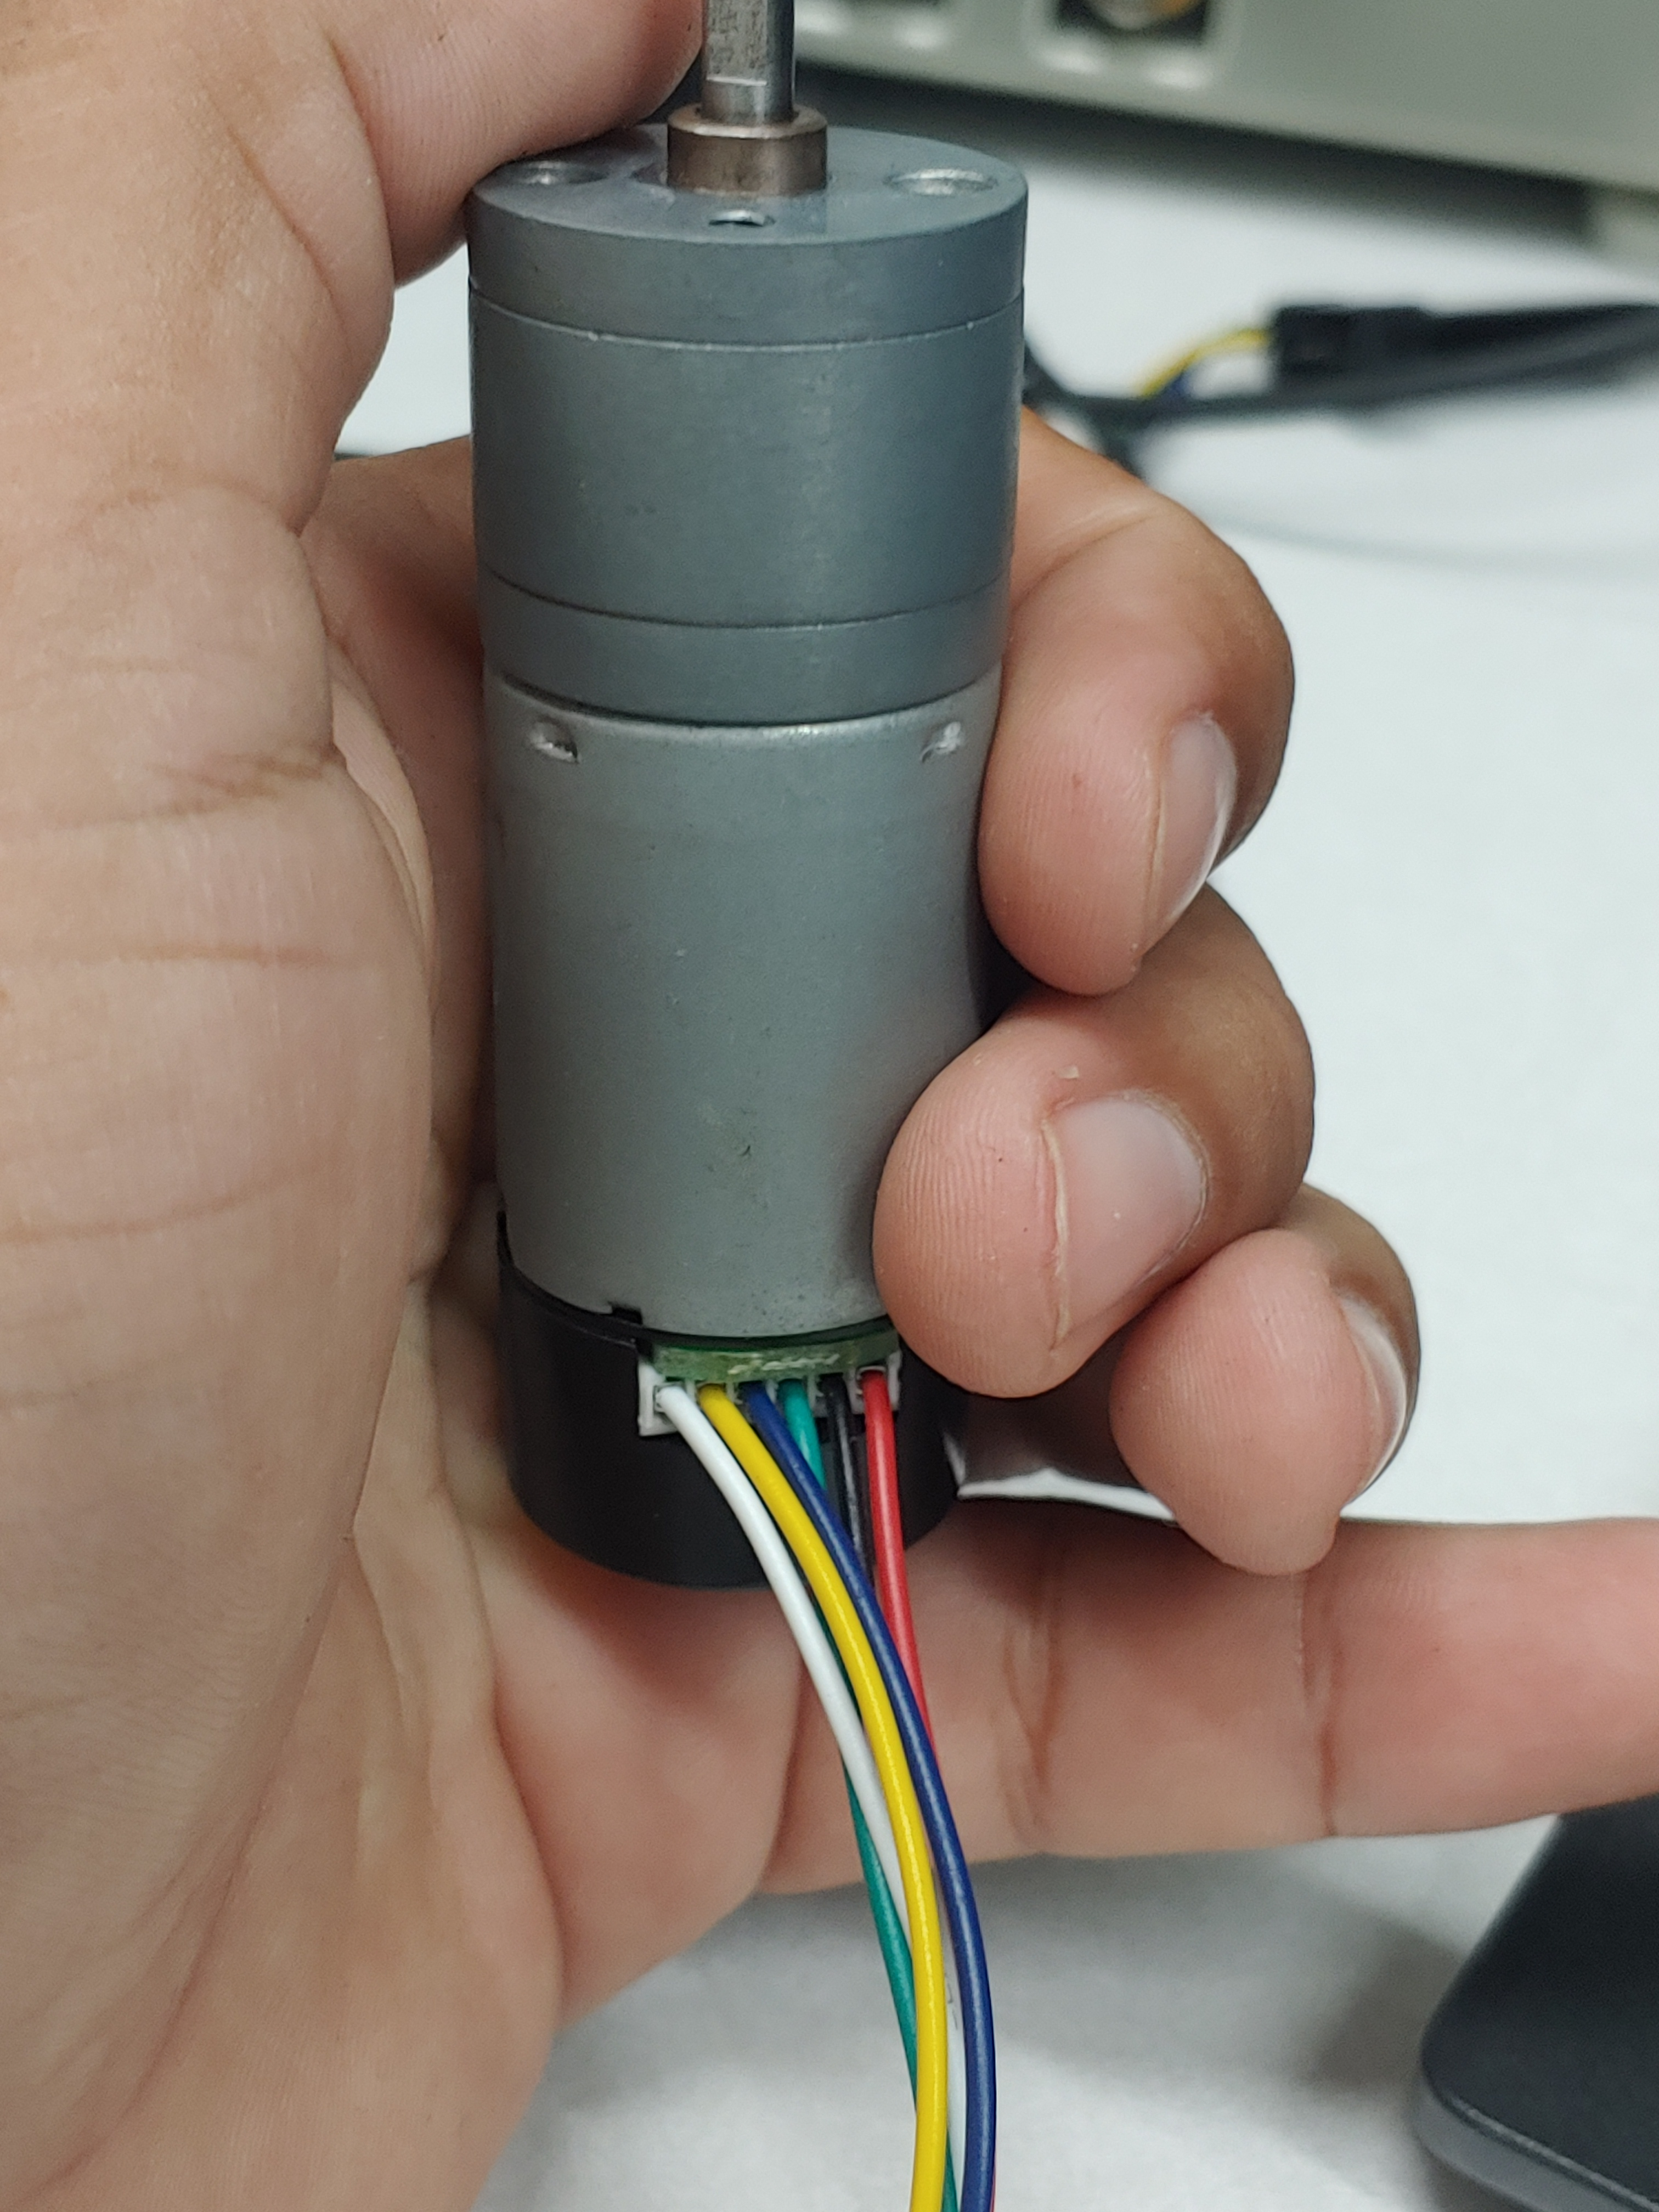
\includegraphics[width=0.30\txw]{Imagenes/motor_1_sensor.jpg}
	\caption{Figura 1: Motor con un sensor de efecto Hall.}
	\label{fig:mot1}
\end{figure}

Para obtener un valor estimado de los pulsos por revolución del motor se puede usar el tamaño del reductor y la resolución del encoder, esta puede variar entre 11 y 12 señales que pueden entregar los canales A y B; los pulsos estimados son el producto del tamaño en el reductor y la resolución del encoder.

En caso de calcular la velocidad y posición de un motor con dos sensores Hall (o uno solamente para la velocidad) primero se deben de calcular los pulsos por revolución que hay en una vuelta (360°), con base al valor obtenido se pueden convertir los pulsos en velocidad. Considerando que se usará un microcontrolador para realizar este conteo de pulsos conviene hacer el uso de interrupciones para contar con precisión los pulsos generados en 360 grados y mostrar los valores sondeados en texto a través de la comunicación en serie que integra el microcontrolador. 

La conexión necesaria para hacer el conteo de los pulsos con el microcontrolador consiste en conectar el canal A del encoder en un pin del microcontrolador que admita interrupciones, luego se conecta el VCC y GND del encoder a los pines de alimentación en el microcontrolador o se puede alimentar con una fuente externa.

Una vez que obtenida la cantidad de pulsos que hay en una vuelta se puede calcular la velocidad y posición del motor a través de las siguientes fórmulas:

\begin{equation}
\begin{aligned}
	\omega_{RPM} &= \frac{60V_s}{Cnt}\\
	\omega_{rad} &= \omega_{RPM}\frac{\pi}{180}\\
	\omega_{gr} &= \omega_{rad}\frac{180}{\pi}
\end{aligned}
\end{equation}

donde, $V_s$ es la velocidad del motor muestreada.
Para detectar la posición del motor (si va a derecha o izquierda) es necesario que este cuente don dos sensores de efecto Hall, ya que con estos se tiene un encoder de cuadratura, donde una de los dos señales del codificador se desfasa 90°. Con esta información se puede determinar si el motor gira en sentido horario o antihorario, adelantándose el canal A respecto al B se toma que el motor gira a la derecha (horario), si el canal B se adelanta entonces toma que el motor va a la izquierda (antihorario).

Si se desea analizar el comportamiento del encoder que integra el motor con un osciloscopio entonces se debe de alimentar este con 3.3V o 5V, obtenibles desde un microcontrolador como el Arduino, y conociendo qué canal corresponde a cada cable conectar el gancho de la sonda en uno de los canales a observar, seguidamente conectar el caimán que sale de la sonda a tierra, igual obtenible desde el Arduino. No hace falta hacer funcionar el motor ya que se puede hacer girar el reductor manualmente para ver los pulsos que genera.

\begin{figure}[H]
	\centering
	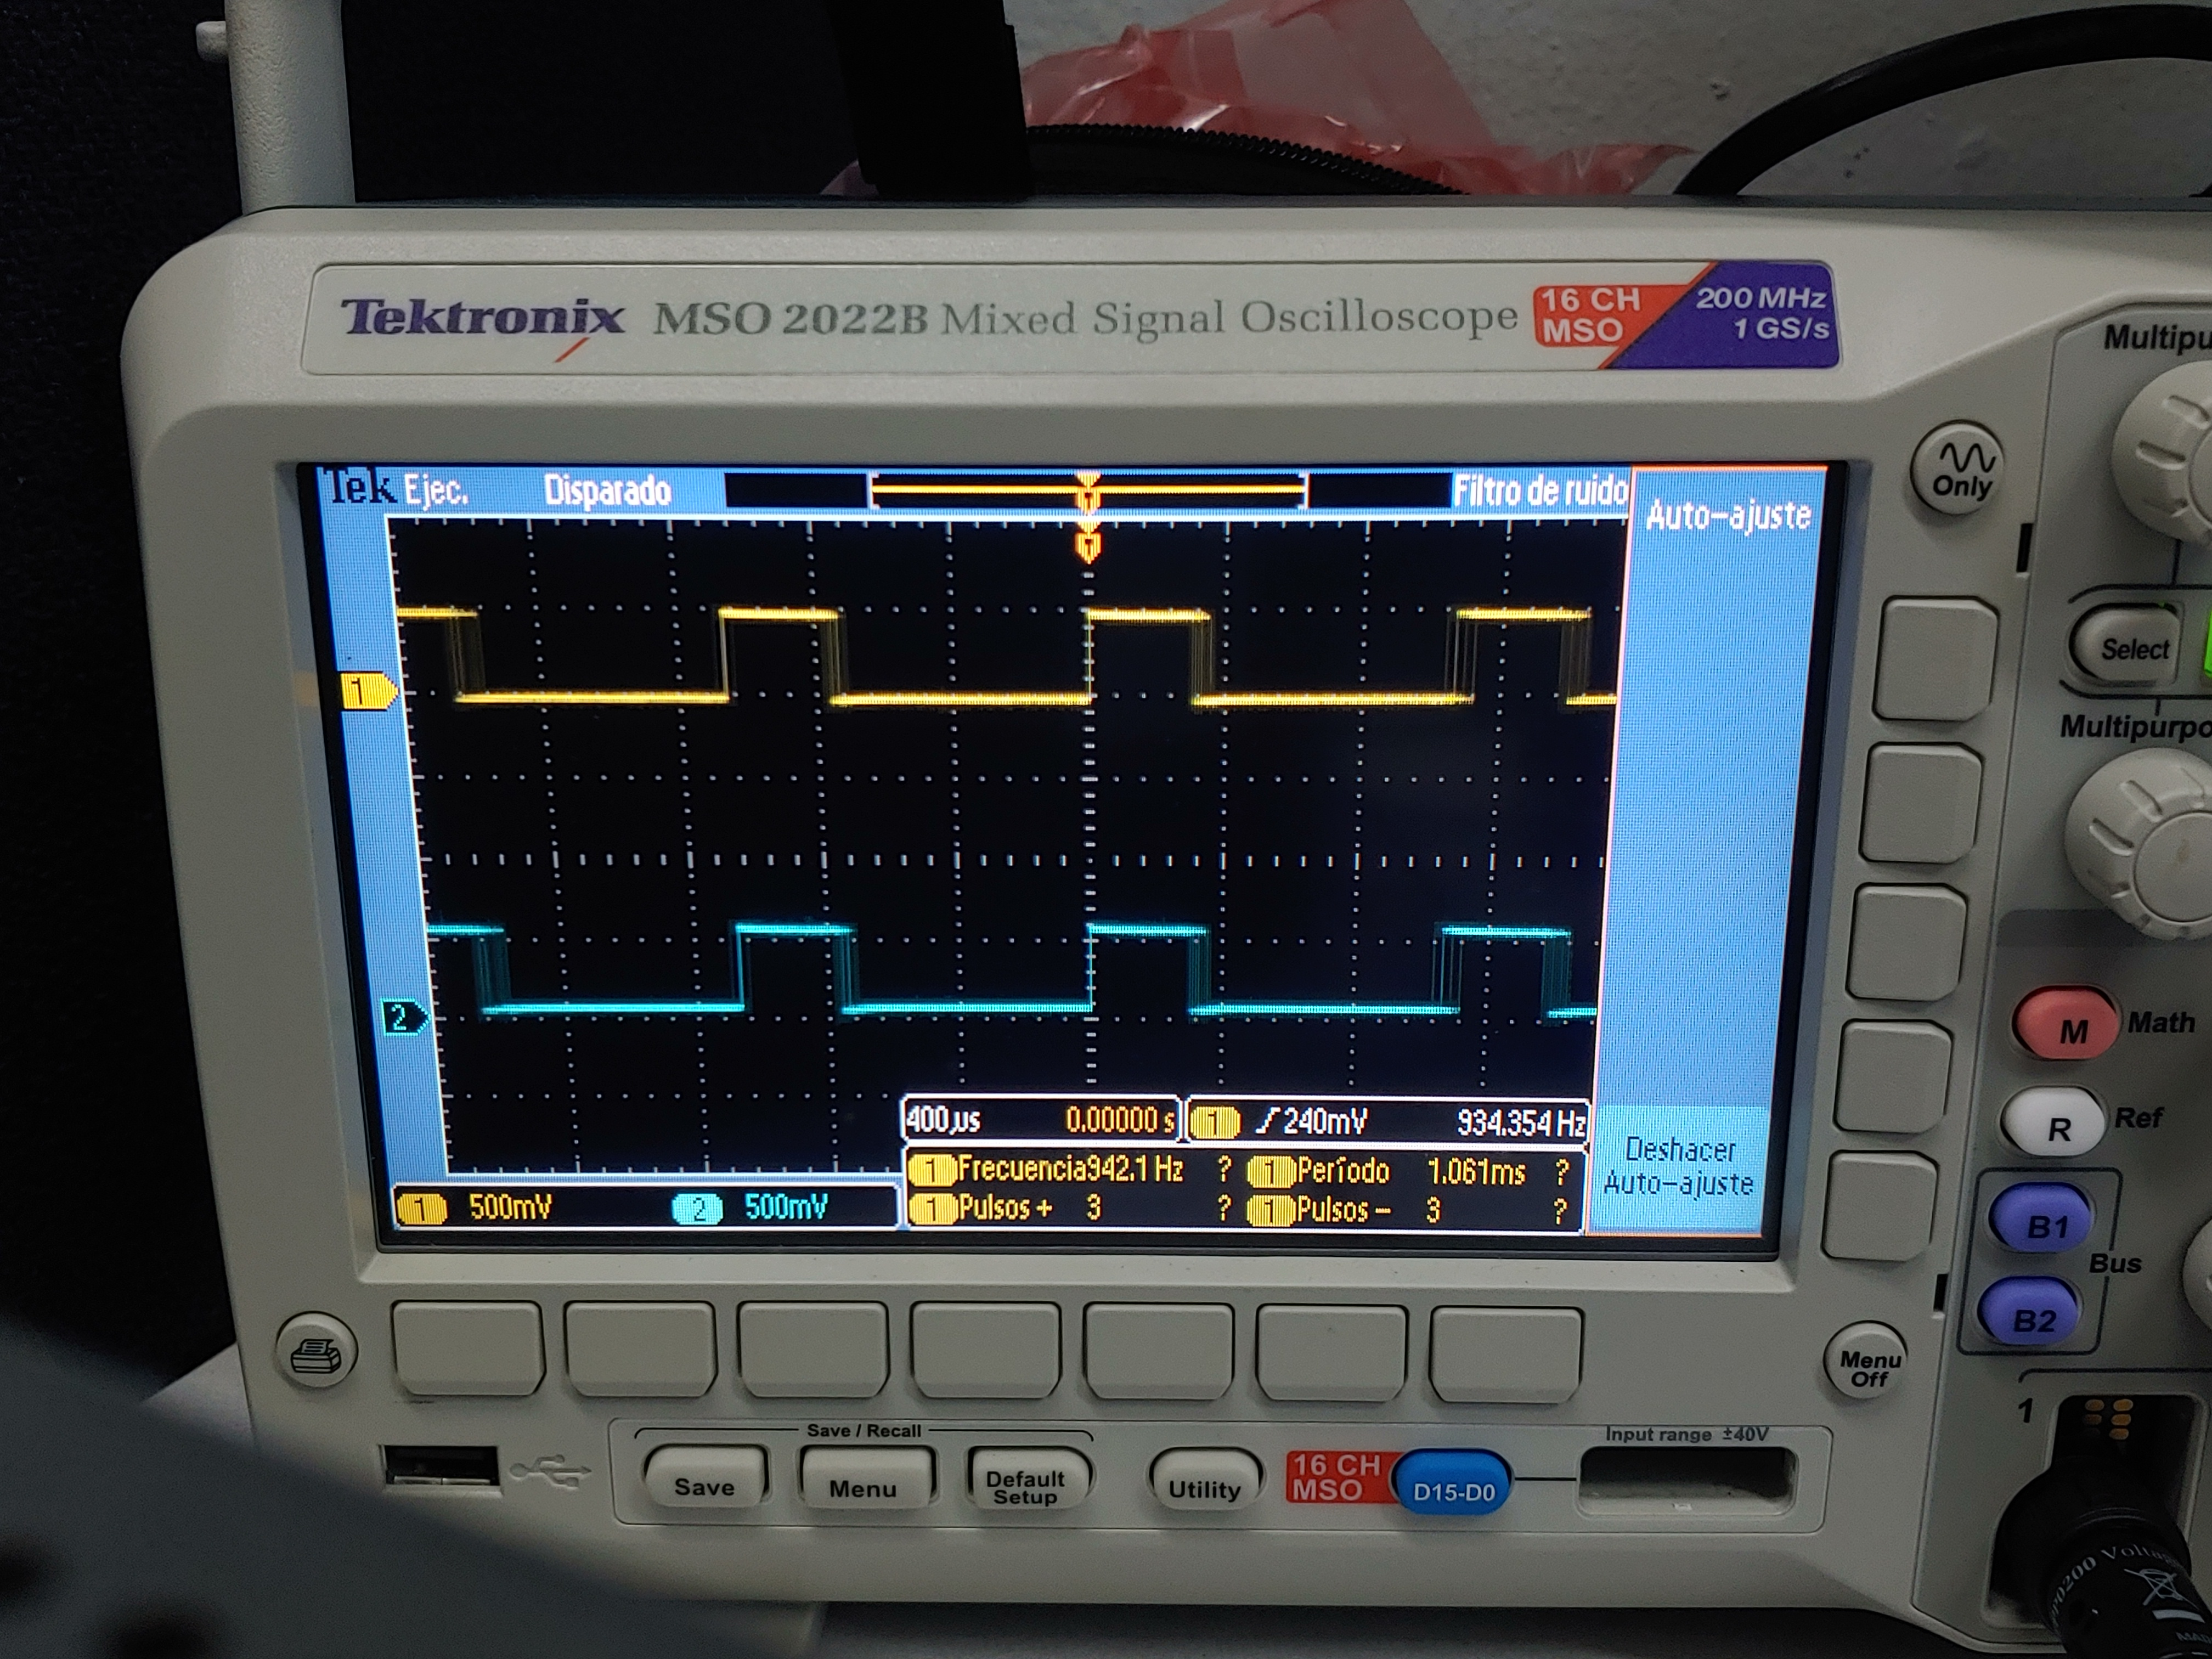
\includegraphics[width=0.40\txw]{Imagenes/Osciloscopio.jpg}
	\caption{Imagen 2: Señal del encoder vista con el osciloscopio.}
	\label{fig:Oscilo}
\end{figure}

Las señales observadas en la Imagen~\ref{fig:Oscilo} corresponden al motor con sin encoder de cuadratura, debido a la falta de un segundo sensor de efecto Hall para detectar el sentido de giro, las señales para un codificador de cuadratura se observan de la siguiente manera:

\begin{figure}[H]
	\centering
	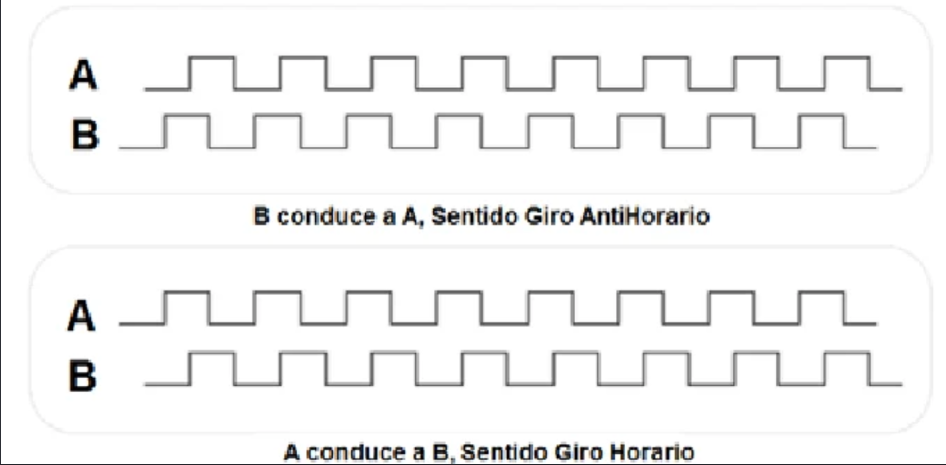
\includegraphics[width=0.40\txw]{Imagenes/cuadratura.png}
	\caption{Imagen 3: Señales de un sensor con cuadratura.}
	\label{fig:cuadratura}
\end{figure}

\end{linespacing}





En la sección~\ref{sec:Motor} (que es esta)

En este trabajo citamos los siguientes artículos: \cite{Kerr2010}, \cite{Schanda2007}.

También puedes escribir algo así como ``vease la sig referencia~\citep{Kerr2010}'', o también puedes usar citet: ``vease la sig referencia~\citet{Kerr2010}''.

\bibliography{referencias}

}
\end{document}

%%% Local Variables: %%% mode: latex %%% TeX-master: t %%% End:
